\documentclass[senior]{IPSstyle}

  \Year{2018}
  \Month{September}
  \Author{44161580-4: JIN YUTING}

  \Title{Flight schedule recovery with ant colony optimization}

  \Advisor{Professor Fujimura}

\usepackage{amssymb,amsmath}

\usepackage{mathptmx}
\usepackage{helvet}
\usepackage{courier}
\usepackage{type1cm}

\usepackage{makeidx}
\usepackage{graphicx,subfigure}
\usepackage{multicol}
\usepackage{multirow}
\usepackage[bottom]{footmisc}

\usepackage{mathrsfs}
\usepackage{amssymb,amsmath}
\usepackage{amsfonts}
\usepackage{color}
\usepackage{CJKutf8}

\usepackage{listings}
\usepackage{algorithm,algorithmicx,algpseudocode}
\usepackage[toc,page,title,titletoc,header]{appendix}

\renewcommand{\algorithmicrequire}{\textbf{Input:}}
\renewcommand{\algorithmicensure}{\textbf{Output:}}

  \Abstract{
In computer vision\cite{witten2016data}, object boundary is defined as the enclosed set of edge pixels by which an object is tightly surrounded. Given the object boundary, the shapes and locations of the objects in an image can be easily recognized. However, object boundary detection is still a challenging problem due to the multi-scale object problem, the interference caused by the local edges with less semantic information, and the large variance of backgrounds and scenes. In this thesis, we develop a cascaded framework to improve the performance of the present edge detection algorithms in object boundary detection. Within our framework, present networks can be cascaded one-by-one and trained end-to-end to gain more semantic information from the inputs. We test our method in two scenes: neuronal boundary detection in Electron Microscopy (\emph{EM}) images, and object boundary detection in natural images. Massive experiments and analyses show that the proposed cascaded fully convolutional networks can exactly outperform the competitors with the help of the cascaded structure.
}

\Keywords{Fully Convolutional Networks, Object Boundary Detection, Neuronal Segmentation, Cascaded Structures}

\Acknowledgments{

One year ago I chose to leave home and come here with the encouragement from my family, which took the most memorable days in my life to me. So firstly, I would thank my mother and father for their comprehension and supports.

I would express my sincere thinks to Professor Jinglu Hu. Professor Hu is a warm-hearted supervisor who always provides the guidance and suggestions on me, and a rigorous researcher. Without the insightful suggestions and kind reminders from Professor Hu, there might be a hard time for me especially in the days of graduating. 

I would also appreciate Dr. Shen, my supervisor in Shanghai University for teaching me the basic scientific accomplishment and providing me inspirations on the research. 

Thanks my friends who lended me a hand when I went into troubles.

Thank you all!



}


\begin{document}

 \makepreliminarypages
 \singlespace
 \frontmatter
 \tableofcontents
 \listoffigures
 \listoftables
 \mainmatter
 \clearemptydoublepage
 \setlength{\baselineskip}{23.0pt}

\chapter{Introduction} \label{introduction}



\section{Background}

\subsection{Current status of Chinese Aviation Industry}
In recent years, as an efficient transportation tool, airplane becomes a more and more common choice for travelling people. Statistics shows that in 2017 the number of passengers traveling by airplane is up to 4100 million worldwide. 
Since 1980s, Chinese civil aviation industry has been developing dramatically. 
From 2017 Civil Aviation Industry Development Statistics Bulletin, the total transport turnover volume was 1083.08 billion ton-kilometers, up 12.6\%, passenger transport volume was 9513.04 billion person-kilometers, up 13.5\%, and postal delivery volume was 243.55 billion ton-kilometers, up 9.8\%, compared with the data in 2016. 
In the past five years, the major transport indicator of Civil Aviation Administration of Chinese all increased with a dramatic speed, much higher than other transportation modes and average China's GDP growth level.

However, the rapid development of the civil aviation industry has also led to the increasingly serious flight delays.
Compared with developed country, Chinese civil aviation has higher flight delay frequency, longer delay time, more disputes between airline companies and passengers.
In the first two quarters of 2017, the average flight punctuality rate of Chinese Civil Aviation was 66.22\%, slipped 9.27\% year-on-year, with an average delay of 30 minutes, increased 11 minutes compared with the same period last year. With the influence of summer weather, the alignment rate dropped to 50\%.
Meanwhile, the total number of complaints received in 2017 increased by 29.3\% over the same period last year.
Therefore, flight delay problem of Chinese civil aviation has become an industrial public problem, which has led to a broad and sustained attention of the whole society.

In such circumstances, for Civil Aviation Administration Department of China and aviation transport enterprise, it has becomes an urgent problem to consider that how to control flight delay, improve flight punctuality rate and resolve disputes between passengers and airline companies caused by flight delays.

\subsection{Causes of flight delay}
In daily operation of airline company, flight delays are happening almost everyday.
According to the regulations on the normal statistics of civil aviation flights, flight delays are defined as:
\begin{itemize}
    \item flights that still did not take off in 15 minutes after the departure time published in timetable.
    \item flights that did not open the hatch at the arrival time published in timetable.
\end{itemize}
For this common phenomenon, there are some mean reasons. 

Weather factors, which cause the most frequent flight delays, should be considered first. 
Bad weather such as thunder, rain, fog and so on is force majeure events which is unpredictable and unavoidable. 
However in actual operation, fine weather at departure airport doesn’t mean flights can take off successfully. 
Weather factors are usually analyzed at three points.
\begin{enumerate}
\item Whether the weather condition of departure airport is suitable for take-off. 
\item Whether the weather condition of destination airport is suitable for landing.
\item Whether the weather condition during the flight route is suitable for flying.
\end{enumerate}

In addition, even for same aircraft type, different airlines has great differences in specific safety standards.
And whether the flight will take off is also dependent on captain's judgment. 
The captain's decision on the current aircraft condition, airport and weather is also quite different.

The second leading reason is air traffic control. 
Due to recently explosive growth of air traffic flow, it is difficult for current flight management system to adapt. 
On the one hand, the development of corresponding ground facilities, equipment and service assurance can not keep up with high growth speed of civil aviation industry; 
on the other hand, current air route structure is no longer reasonable for increased air flow. 
So it has to be strictly restricted to the airspace.
And Air Force Activities may also lead to sudden air traffic control. In this case, passenger can only wait, no time to predict.

The third reason is aircraft failure.
Although most of hidden troubles can be dealt with in routine inspection, there is no guarantee that the aircraft equipment won’t suddenly fail. 
In order to ensure safety and completely eliminate hidden dangers, it always causes some delay. 
And if the airport that aircraft failure occurs is not airline’s aircraft maintenance base, the delay time will be so long and can’t be determined, even causes flight cancellations. 

The final reason is about passengers. 
Among all the reasons contributing to flight delay, the human factor of passenger's cause has become a "new growth point".
In order to wait or look around for a few passengers who are late, lost or does not heard of announcement, may also cause flight delays.
And sometimes a few minutes of delay may meet with longer delays caused by weather or air control.

Flight delays caused by reasons above is all dependent delay. In real life, we probably meet the delay caused by preceding flight delay. 
Usually, airlines plan flight schedule ahead of time, and to make profit maximization, they set flight schedule as intensive as possible. 
However, the shortage is that reduces robustness of whole airline network. With high density scheduling, once accidents occur, coordination becomes difficult.
Any omissions in the preceding flight may trigger a chain reaction of the subsequent flights. and the later flight is, the longer its delay time will be.
This kind of delay is going to be a more and more serious problem that forces airlines to confront.

%%%%%%%%%%%%%%%%%%%%%%%%%%%%%%%%%%%%%%%%%%%%%%%%%%%%%%%%%%%%%%%%%%%%%%%%%%%%%%%


\section{Motivation}
The operating goals of airline companies is reducing costs and improving profits as much as possible.
But accidents may disrupt original flight schedule, and cause economic losses to airline companies.
For airline, this loss can be divided into direct and indirect part.

Direct economic losses include loss of flight delay in ground-holding, loss of delay caused by air traffic jam, cost of accommodation for stranded passengers caused by long time delay or flight cancellation, and cost of temporary aircraft deployment. These extra costs directly increase airline company’s operation cost. 

In addition, flight delays also affect airline’s normal profit, cause indirect loss to airline company.

And for passengers, flight delay is also unpleasant experience. Flight delays or cancellation waste passenger’s private time and disrupt travel plans.

Besides huge economic losses for the airlines, flight disruption also bring great challenges to the normal operation of airports. Large scale of flight delays would disrupt airport running scheduling and cause a series of chain reactions. 

Therefore, when flight schedule was disrupted, how to make rescheduling in a short time has become an urgent need for the civil aviation industry. Rescheduling means to make a new schedule of affected flights based on original timetable.  The target is not only schedule the delayed flights with the best scheme, but also use as less time as possible. The rapider the recovery could be, the more the flight delay accumulation and the economic loss can be reduced.

%%%%%%%%%%%%%%%%%%%%%%%%%%%%%%%%%%%%%%%%%%%%%%%%%%%%%%%%%%%%%%%%%%%%%%%%%%%%%%%

\section{Organization of the thesis}
The rest of this thesis is structured as follows: Chapter 2 introduces some related works of past research in flight disruption management area. Chapter 3 I introduce the application of ant colony optimization which is the main method of solving flight rescheduling problem, including the novelty of my research. In Chapter 4 I will explain implement of ant colony optimization including evaluation process. And Chapter 5 is experiment using real world data. The last part, Chapter 6 describes the conclusion and future works of this research.

%%%%%%%%%%%%%%%%%%%%%%%%%%%%%%%%%%%%%%%%%%%%%%%%%%%%%%%%%%%%%%Chapter 3
\chapter{Related Work} \label{related_work}
%%%%%%%%%%%%%%%%%%%%%%%%%%%%%%%%%%%%%%%%%%%%%%%%%%%%%%%%%%%%%%Chapter 3


%%%%%%%%%%%%%%%%%%%%%%%%%%%%%%%%%%%%%%%%%%%%%%%%%%%%%%%%%%%%%%%%%%%%%%%%%%%%%%%




%%%%%%%%%%%%%%%%%%%%%%%%%%%%%%%%%%%%%%%%%%%%%%%%%%%%%%%%%%%%%%%%%%%%%%%%%%%%%%%


\chapter{Methodology} \label{methodology}

\section{Data preprocess}

In this research, we get a dataset of original flight schedule from airline company at beginning.
This dataset includes flight id over a period of time, with its corresponding departure time and airport, landing time and airport, aircraft id and passenger information.
We consider a typical disruption like airport closure. 
It usually occurs unpredictably, and once it occurs, the closed airport will limit either departure or landing activities.
So when the bad weather causes airport closure, we suppose that airline company has internal notice of closure before real closure time for captains to react and we assume notice time is one hour earlier than closure time.
For optimization process, we intercept the flights from notice time to the end of that day.
Cause flight schedule is disrupted by one airport closure, we develop some rules for data preprocess before optimization process.
\begin{enumerate}
    \item Flights limitation: airport closure limits aircraft departure, so the flights which departure from closure airport with departure time after closure time will be cancelled.
    \item Aircraft availability: at the notice time, some aircraft have already been in mid-flight. For these aircraft, they will be available again after finishing current flight. The available time of these aircraft will be the landing time of their current flight, in the airport of their current flights’ landing airport.
    
    But there is a special series of aircraft should be considered. These aircraft departure before notice time so their captain will receive notice of airport closure during mid-flight. However, because these flights are scheduled to land at closed airport after closure time, they have to fly back to departure airport, and these aircraft can used again at 
    \begin{equation*}
    notice\_time+(notice\_time-departure\_time.)    
    \end{equation*}
\end{enumerate}

With this preprocess above, we can get a list of flights remained and a series of aircraft available. With these two dataset, we can get the relationship between aircraft and flights and then create elicitation factor table. The specific operation methods will be explained in section 4.

\section{Adjustment and evaluation}

\subsection{Flight adjustment method}
When a scheduled flight timetable is disrupted, for example, the bad weather causes airport closure or aircraft failure happens, we need to adjust the following flights. In general, there are some typical methods for adjustment.
\begin{enumerate}
    \item Adjust following flights’ departure time. This method can be considered as we allow delay in adjustment. Sometimes, delay is unavoidable, but we can make it as less as possible.
    \item Cancel the flight. In some circumstance, cancelling a flight and arrange redeeming flight on the next day will be better than delay for a long time. This is a method to make more reasonable use of resource.
    \item Change original aircraft-flight set. This means we assign a flight to an aircraft which different from the one on original schedule. Cause some aircraft may be spare and can be arranged for extra flights, this measure can utilize aircraft resource more effective.
    \itemTransfer aircraft from other airports. In actual, this is not a common approach. Transferring means the aircraft need to take a flight with no passenger, so this method is only used when the disrupted flight is so important that cannot be cancelled. 
\end{enumerate}
%%%%%%%%%%%%%%%%%%%%%%%%%%%%%%%%%%%%%%%%%%%%%%%%%%%%%%%%%%%%%%%%%%%%%%%%%%%%%%%

\subsection{Objective Function}
In this research, we use total cost to evaluate each feasible solution. When a new feasible timetable be scheduled, the total cost can be calculated as below.
\begin{equation}
    Total\ cost=C_a+C_d+C_c+C_p
\end{equation}
\begin{equation}
    C_a = \sum_{f\in F} x_{f}*P_1
\end{equation}
\begin{equation}
    C_d =\sum_{f\in F} T_{d_f}*P_2
\end{equation}
\begin{equation}
    C_c=\sum_{f\in F} z_{f}*P_3
\end{equation}
\begin{equation}
    C_p=\sum_{f\in F} y_f*T_{d_f}*NP_f*P_4+\sum_{f\in F} z_f*NP_f*P_6+\sum_{f\in F} (y_f+z_f)*CP_f*P_6
\end{equation}

\begin{table}
\renewcommand{\arraystretch}{1.0}
\caption{Parameters and Variables}
\label{piriform_dataset}
\begin{center}
\begin{tabular}{|c|c|}
\hline
\multicolumn{1}{|c|}{Var}
&\multicolumn{1}{c|}{Meaning}
\\
\hline
\(A\)	&	Set of all aircraft \(a\)
\\	\hline
\(F\)	&	Set of all flights \(f\)
\\	\hline
\(C_a\) &   Cost of changing aircraft.
\\  \hline
\(C_d\) &   Cost of delay.
\\  \hline
\(C_c\) &   Cost of cancellation.
\\  \hline
\(C_p\) &   Cost of passenger satisfaction.
\\  \hline
\(x_f\)	&   \(=0\), if flight\(f\) assigned to the same aircraft as original schedule; \(=1\), if not.
\\	\hline
\(y_f\) &   \(=1\), if flight\(f\) is delayed; \(=0\), if not.
\\  \hline
\(z_f\) &   \(=1\), if flight\(f\) is cancelled; \(=0\), if not.
\\  \hline
\(T_df\) &   The total delay time of flight\(f\) (minutes).
\\  \hline
\(NP_f\) &  Total number of passengers on flight\(f\).
\\  \hline
\(CP_f\) &   Number of passengers following with connecting flight on flight\(f\)
\\  \hline
\(P_1\) &   Cost of changing original aircraft for one flight.
\\  \hline
\(P_2\) &   Cost of delay for one flight per minute.
\\  \hline
\(P_3\) &   Cost of cancelling one flight.
\\  \hline
\(P_4\) &   Cost of maintaining passenger satisfaction for delaying flight per minute per passenger.
\\  \hline
\(P_5\) &   Cost of  maintaining passenger satisfaction for cancelled flight per passenger.
\\  \hline
\end{tabular}
\end{center}
\end{table}

Based on the one in \cite{sousa2015airline}, the module in this research made some change. Corresponding to different adjustment method, the total cost is divided into four parts fig.\ref{fig:cost structure}: cost of changing aircraft, cost of delay, cost of cancellation and cost of passenger satisfaction maintenance. Evaluation is in airline company’s view, so the passengers’ satisfaction can be quantified as a kind of cost. And in this part, we consider a special class of passengers with connecting flights. These passengers purchase more than one tickets at one-time and need to take a transit in midway. So it will do great effect on the rest of their journey if the first flight in connecting flights is delayed. There will also be probably for them to miss the next flight. 

To calculate the cost of part, we need to know the status of each flight in new feasible solution. 
In this research, there are three indicators to represent the three flight status: changed aircraft, delayed, cancelled. 

\begin{figure}[t]
    \centering
    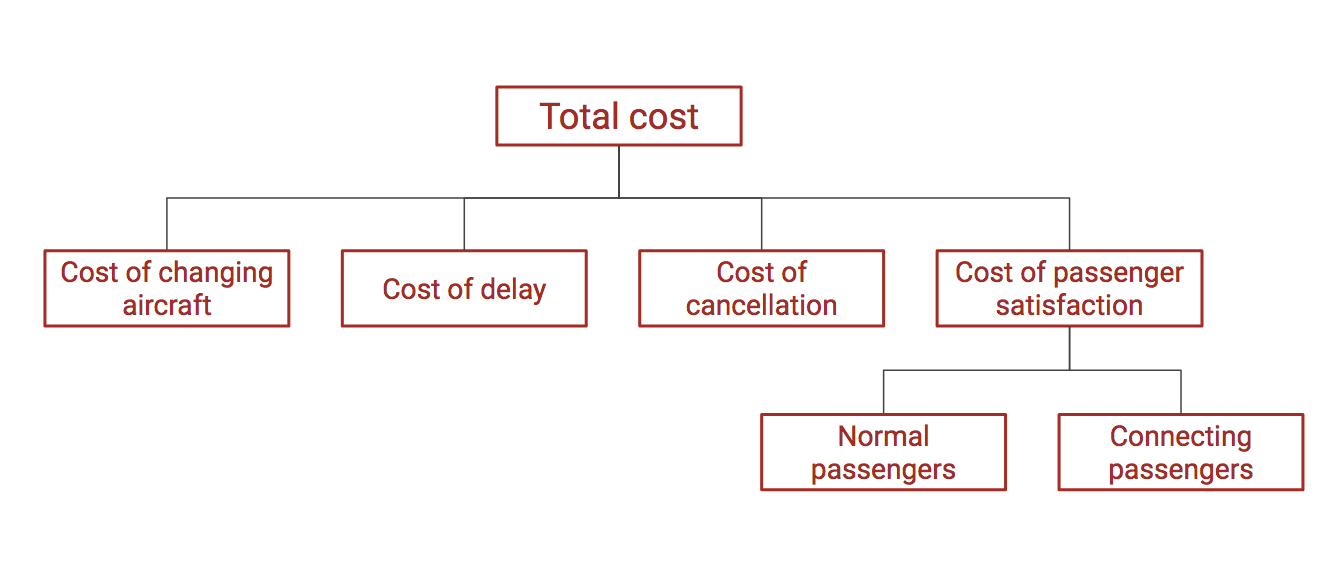
\includegraphics[width=300]{MasterThesis-master/Coststructure.png}
    \caption{Structure of total cost}
    \label{fig:coststructure}
\end{figure}

\(x_f\) indicates the status that if the flight \(f\)is assigned to the same aircraft as original schedule. \(y_y\) indicates the status that if the flight \(f\) is delayed. And \(z_f\) indicates the status that if the flight \(f\) is cancelled. \(x_f\), \(y_f\) and \(z_f\) is Boolean value(0 or 1).
%%%%%%%%%%%%%%%%%%%%%%%%%%%%%%%%%%%%%%%%%%%%%%%%%%%%%%%%%%%%%%%%%%%%%%%%%%%%%%%
\section{Ant colony optimization} \label{Ant colony optimization}

In my research, I apply ant colony optimization for flight rescheduling problem. And in evaluation part, I use cost to measure feasible solutions of each iteration. I build the model based on past thesis and enlarge the scope of the problem. I will explain specifically below. 

\begin{figure}[h]
  \centering
  % Requires \usepackage{graphicx}
  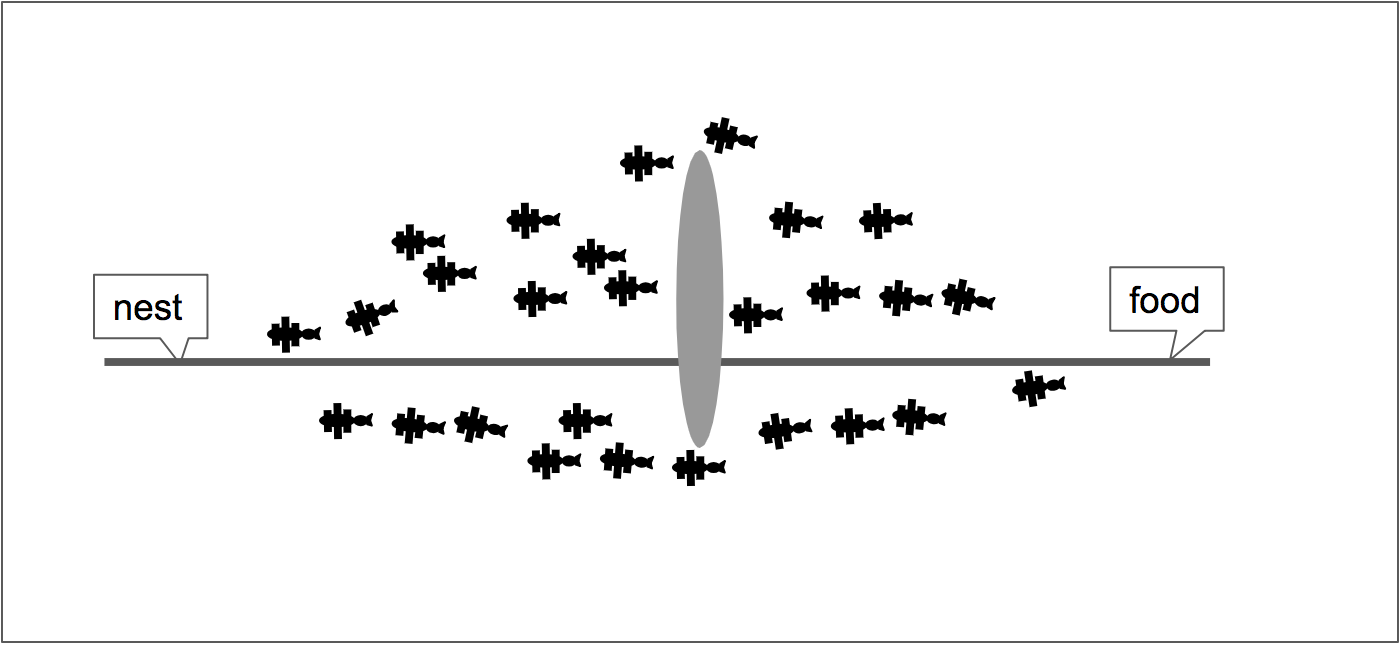
\includegraphics[width=15cm]{MasterThesis-master/ACO-1.png}\\
  \caption{At beginning ants choose paths randomly.}\label{fig: aco1}
\end{figure}
\begin{figure}[h]
    \centering
    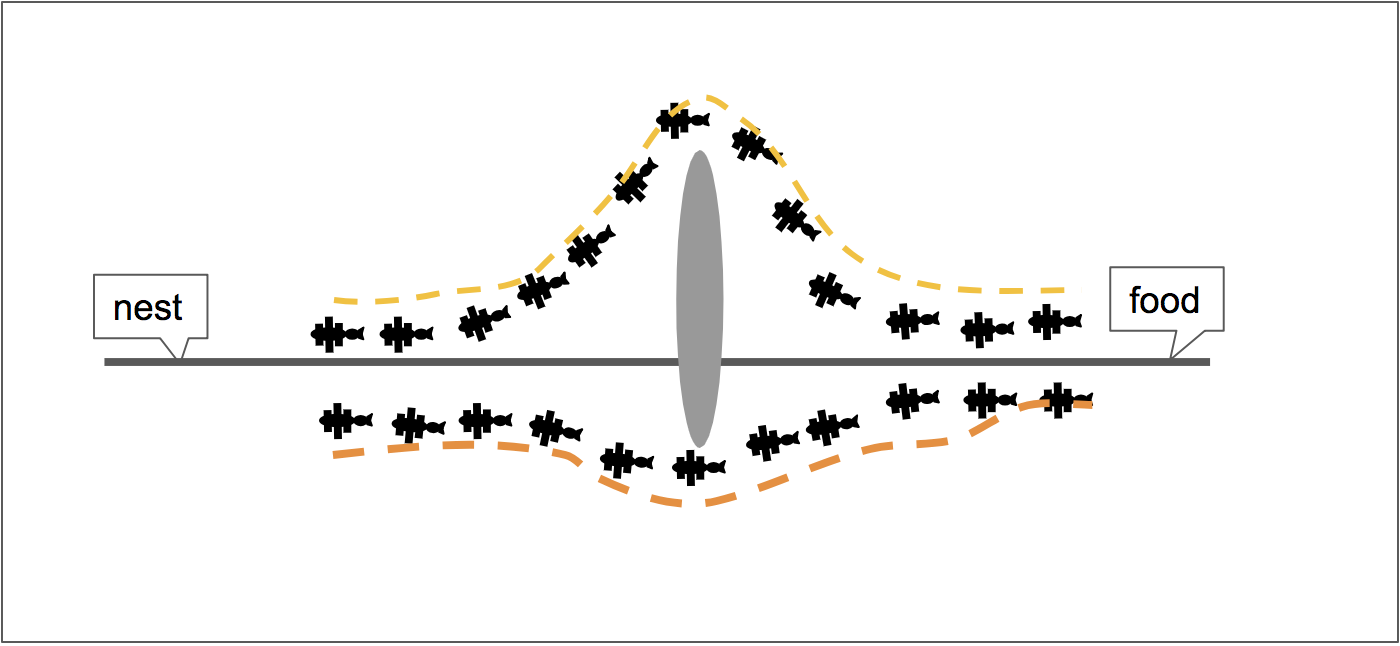
\includegraphics[width=15cm]{MasterThesis-master/ACO-2.png}
    \caption{Ants leaves pheromone on the paths passed.}
    \label{fig:my_label}
\end{figure}
\begin{figure}[h]
    \centering
    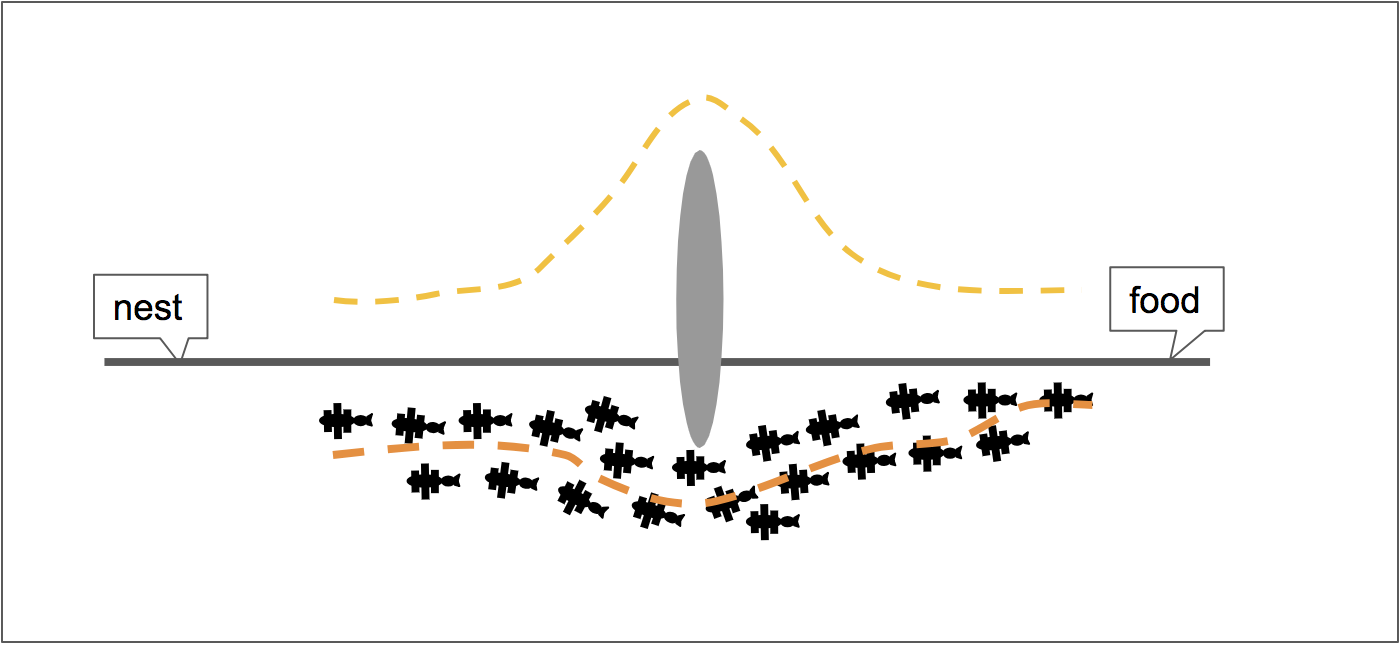
\includegraphics[width=15cm]{MasterThesis-master/ACO-3.png}
    \caption{Finally ants will find optimum route with higher pheromone concentration.}
    \label{fig:my_label}
\end{figure}

As a meta-heuristic algorithm, ant colony optimization is an optimization algorithm simulating foraging behavior of ants. The basic principle of ant colony algorithm is:
\begin{enumerate}
    \item During foraging process, ants release pheromones on the passed path.
    \item When an ant meets an intersection that has not yet passed, it will pick one direction randomly. At the same time, the ant releases pheromones on the path.
    \item When ants later met the intersection, they will the path with a higher concentration of pheromone.
    \item The concentration of pheromone is related to the length of path and is inversely proportional to it. The shorter the path is, the higher the concentration can be.
    \item When the number of ant increases, the pheromone concentration on the optimal path is increased.
    \item As time goes on, the whole ant colony finally find the optimal foraging route.
\end{enumerate}

Ant colony algorithm  was used to solve traveling salesman problem at beginning. 
So in my module, I try to use a whole path to represent a feasible schedule solution. 
Considering both flights and aircraft as cities in TSP,  the path between each two cities indicates the relationship between flights and flights or aircraft and flights. 
And in flight schedule problem, the final goal is minimum the whole cost. So when we get a feasible route, we can calculate the total cost and consider it as the distance in TSP.

In this algorithm, for each iteration, we have more than one ants and every ant can be seen as a simple agent. There are some constraints:
\begin{enumerate}
    \item One iteration only allows each ant move one step;
    \item For each step, each ant leaves pheromones on the branches that they pass through;
    \item The probability for ants to choose next node is related to the pheromone concentration contained in the linked branch;
    \item Use tabu list to represent nodes that have been passed.
\end{enumerate}

For basic ant colony algorithm, there are two main process:
\begin{enumerate}
    \item State Transition:
    
    In each iteration, every ant moves one step, the probability of ant \(k\) to move from state \(i\) to state \(j\),can be calculated by this function:
    \begin{eqnarray}\label{probability}
    p_{ij}^k &=&
    \begin{cases}
    \cfrac{[\tau(i,j)]^\alpha +[\eta(i,j)]^\beta}{\sum_{z\in J_k(i)} [\tau(i,z)]^\alpha +[\eta(i,z)]^\beta} &, j\in allowed_k \cr
    0 \cr
    \end{cases}
    \end{eqnarray}
    In this function, \(\tau(i,j)\) means the pheromone concentration on the branch between node \(i\) and \(j\), \(eta(i,j)\) represents the desirability of transforming states.(In TSP it is \(1/distance\), but in this research it is \(1/cost\)). 
    
    \(\alpha\) is heuristic factor, controls influence of residual pheromone concentration. The larger the \(\alpha\) is, the greater the possibility of ants choosing the path they have passed before can be, and The randomness of search will be weakened. \(\beta\) is expectation heuristic factor. When \(beta\)increased, the convergence speed also increased, and the algorithm is more likely to fall in local optimum. 
    Usually, the range of \(\alpha\)is \([0,5]\), and the range of \(\beta\) is  \([0,5]\).
    \item Pheromone Update
    
    For process of updating pheromone matrix, there have been three modules.
    \begin{itemize}
        \item Ant-Cycle module:  The increment of pheromone is related to the whole route of search, not related to the specific path choice. This approach updates pheromone amount of all paths on the route after completing a complete path search. It is a global updating method.
        \item Ant-Quantity module: The increment of pheromone is related to the distance of specific path(i,j). This approach is a local updating method and updates pheromone amount on the path after each step of ants.
        \item Ant-Density module: The increment of pheromone is fixed and is also a local updating method.
    \end{itemize}
    In this research, cause the cost can only be calculated after we get a complete fleet schedule, I choose global updating method for each iteration.
    
    And at time \((t+n)\), the pheromone concentration on the path\((i,j)\) can be calculated as:
    \begin{equation}
        \tau _{ij}(t+n)=(1-\rho)\cdot \tau _{ij}(t)+\Delta\tau _{ij}(t)
    \end{equation}
    \begin{equation}
        \Delta\tau _{ij}(t) = \sum_{k=1}^m \Delta\tau _{ij}^k(t)
    \end{equation}
    \(\rho\) represents the evaporation factor. If \(\rho\) is too small, the pheromone remained on each path will be too much, and influence the convergence speed; but if \(\rho\) is too big, some effective path will be skipped. 
    
    \(m\) is the total number of ant colony. The larger the \(m\) is, the  more accurate the result will be. But if the \(m\) is too big, it will slow down the speed of computing.
\end{enumerate}

 


\section{Innovation} \label{innovation}
In this module, we try to widen the scope of flight recovery problem with application of ant colony optimization. H. Sousa(2015) considered a disruption scenario of aircraft failure during a time period. In this research, we consider a more complicated circumstance of airport closure which is also more close to reality. When airport closure (usually caused by bad weather) happens, it will influence a series of flights and limit aircraft’s departure and landing. The challenge is this problem involves a large number of flights and status of flight and aircraft is changing over the time. So we insert data preprocess, to divide these flights and aircraft into different situations and handle them separately. 

Another improvement is that we divide passengers into two parts and consider those passengers buy connecting flights. In past thesis, maintaining passengers’ satisfaction is considered as an important influencing factor, but it always to be analyzed as a whole unit. In this research, we think passengers with connecting flights are special, because if the delayed or cancelled flight is their first flight of connecting tickets, they will suffer greater impacts than other passengers. So in this module, no matter the flight is delayed or cancelled, we assume that the passengers with connecting tickets on this flight cannot catch the next flight. So that delaying or cancelling flights with connecting passengers will have higher punishment and cost more.

For algorithm, we add randomness in selecting next node part. In each iteration, every ant creates its own route and it chooses the next node by probability. This probability is calculated by the pheromone value on the path connecting the current node and the next one. However, it we only use this rules, ants will more likely to choose the path that have been past before. So we insert some randomness into selecting process. In this way, ants will have more probability to choose path randomly in the first couple of iteration, and the algorithm can avoid falling into local minimum too fast.


%%%%%%%%%%%%%%%%%%%%%%%%%%%%%%%%%%%%%%%%%%%%%%%%%%%%%%%%%%%%%%%%%%%%%%%%%%%%%%%


\chapter{Implement} \label{implement}
In this section, I will explain the specific step of optimization process and use a couple of flights as an example. At the beginning of the whole process, the input is original flight schedule and disruption scenario includes the time and location of occurrence. And our goal is to output a feasible solution with fitness which is total cost in this model as less as possible using ant colony optimization.

\section{Preparation}

In preparation part, we need to preprocess the dataset. At the beginning, we get an original schedule form over a period of time, some days or one month. This form includes too much information so that will be difficult to use this dataset for following computing. So we create another two form based on this original one. The first is flight information dataset, which includes flights’ id, departure and landing time, departure and landing airport, the number of total passengers and passengers with connecting tickets, total flying time and original aircraft pair. Second one is aircraft status dataset, which records the status of each aircraft at the process beginning moment, includes aircraft's id, available time, current location and available seats number.

\begin{table}[t]
\renewcommand{\arraystretch}{1}
\caption{Flight information}
\label{Flight_information_dataset}
\begin{center}
\begin{tabular}{|c|c|}
\hline
\multicolumn{1}{|c|}{Attribute}
&\multicolumn{1}{c|}{Meaning}
\\
\hline
\(flight\_id\)	&	Unique for each flight
\\	\hline
\(departure\_time\)	&	Original departure time
\\	\hline
\(departure\_airport\) &   departure airport, cannot be changed
\\  \hline
\(landing\_time\) &   Original landing time
\\  \hline
\(landing\_airport\) &   Flight's destination
\\  \hline
\(flying\_time\) &   Calculated by its departure time and landing time
\\  \hline
\(num\_passengers\)	&   Number of total passengers on flight
\\  \hline
\(num\_connecting\_passenger\) &   Number of passengers with following connecting flight
\\  \hline
\(aircraft\_id\) &   The original aircraft which flight is  assigned to
\\  \hline
\end{tabular}
\end{center}
\end{table}

\begin{table}
\renewcommand{\arraystretch}{1.2}
\caption{Aircraft status}
\label{Aircraft_status_dataset}
\begin{center}
\begin{tabular}{|c|c|}
\hline
\multicolumn{1}{|c|}{Attribute}
&\multicolumn{1}{c|}{Meaning}
\\  \hline
\(aircraft\_id\)	&	Unique for each aircraft
\\	\hline
\(available\_time\)	&	The time that aircraft can be firstly used(generally is the begin time of process
\\	\hline
\(current\_airport\) &  The location of aircraft at beginning
\\  \hline
\(num\_seats\) &  Accommodating number of this aircraft
\\  \hline
\end{tabular}
\end{center}
\end{table}

Then, we insert disruption scenario. Disruption is reflected as closed airport id and time of closure. To make it more like real life, we suppose a notice time which is the time that airline publish internal closure closure information to captains. We suppose the disruption happens so suddenly that the flights planned to departure before notice time are processed normally. And we use this notice time as the process start time. Using this disruption information, combined with original schedule,  we can get two dataset mentioned above based on the rules below.

Flight information: we only arrange flights in one day.
\begin{enumerate}
    \item intercept the flights which planned to departure after notice time and before the end of the day.
    \item the flights planned to departure after closure time from closed airport are cancelled and remove from dataset.
\end{enumerate}

Aircraft status: we consider notice time as a boundary. 
\begin{enumerate}
    \item If the aircraft is not in flight at the moment of notice time, the aircraft’s available time is notice time, and its current location is landing airport of its last flight. 
    \item For flight on mid-flight at notice time, there are two circumstance.
    \begin{itemize}
        \item If the aircraft originally scheduled to land on closed airport after closure time, this aircraft need to return its departure airport, so its current location is its current flight’s departure airport, and its available time is $notice\_time+ (notice\_time - departure\_time)$
        \item if aircraft’s current flight is not influenced by airport closure, this aircraft’s available time is the landing time of its current flight and current location is landing airport of its current flight.
    \end{itemize}
\end{enumerate}
These two dataset will be the basis of following process.

\section{Relationship}\label{Section4.2}

In this research, we use ant colony optimization as the main algorithm, so there is a key point that we should use a continuous path to represent one feasible schedule solution including both flights and aircraft. The difficult point is how to find feasible path at first. After preprocess, we have flight information dataset and aircraft status dataset. And I will use a small example to explain how to generate feasible paths. 

As shown in Table \ref{Example flight information} and \ref{Example aircraft status}, this example includes six flights and three aircraft.

\begin{table}[h]
\renewcommand{\arraystretch}{1.2}
\caption{Example flight information}
\label{Example flight information}
\begin{center}
\begin{tabular}{|c|c|c|c|c|c|c|}
\hline
\multicolumn{1}{|c|}{flight\_id}
&\multicolumn{1}{c|}{\(f866\)}
&\multicolumn{1}{c|}{\(f874\)}
&\multicolumn{1}{c|}{\(f890\)}
&\multicolumn{1}{c|}{\(f904\)}
&\multicolumn{1}{c|}{\(f2304\)}
&\multicolumn{1}{c|}{\(f2307\)}
\\  \hline
departure\_time & 8:35 & 12:30 & 10:20 & 14:10 & 16:55 & 19:10
\\	\hline
landing\_time & 11:25 & 15:20 & 13:05 & 16:55 & 18:25 & 20:30
\\	\hline
departure\_airport & 49 & 46 & 49 & 46 & 46 & 45
\\  \hline
landing\_airport & 46 & 49 & 46 & 49 & 45 & 46
\\  \hline
flying\_time & 2:50 & 2:50 & 2:45 & 2:45 & 1:30 & 1:20
\\  \hline
aircraft\_id & 42 & 42 & 58 & 58 & 62 & 62
\\  \hline
num\_passengers & 86 & 117 & 114 & 132 & 131 & 107
\\  \hline
num\_connecting\_passenger & 0 & 0 & 0 & 0 & 16 & 58
\\  \hline
\end{tabular}
\end{center}
\end{table}

\begin{table}[h]
\renewcommand{\arraystretch}{1}
\caption{Example aircraft status}
\label{Example aircraft status}
\begin{center}
\begin{tabular}{|c|c|c|c|}
\hline
\multicolumn{1}{|c|}{aircraft\_id}
&\multicolumn{1}{c|}{available\_time}
&\multicolumn{1}{c|}{current\_airport}
&\multicolumn{1}{c|}{num_seats}

\\  \hline
A42 & 8:35 & 49 & 119
\\	\hline
A62 & 8:35 & 46 & 161
\\	\hline
A42 & 8:35 & 49 & 161
\\  \hline
\end{tabular}
\end{center}
\end{table}

\begin{figure}
    \centering
    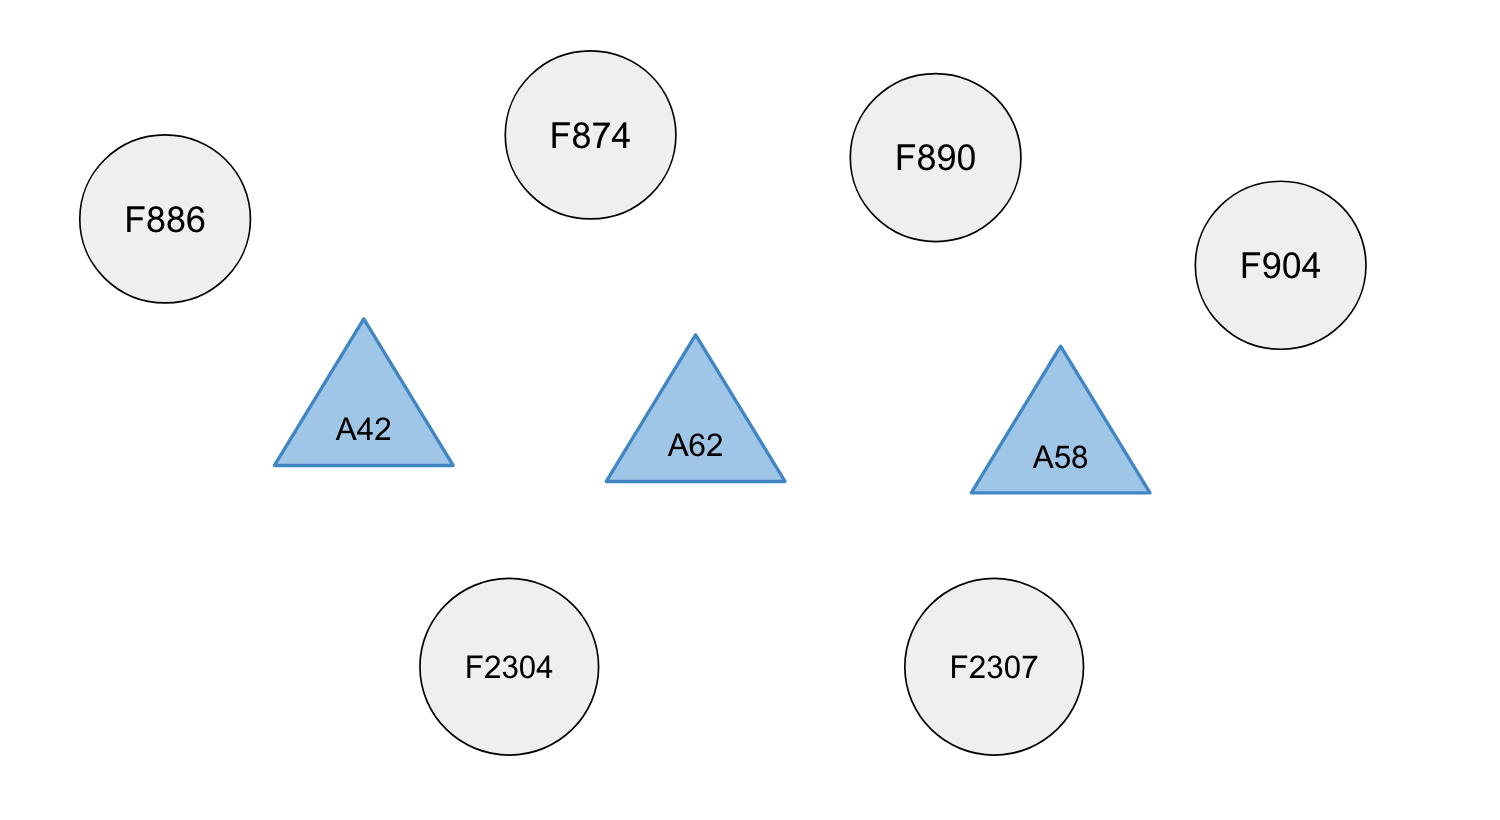
\includegraphics[width=15cm]{MasterThesis-master/nodes.png}\\
    \caption{Aircraft nodes and flight nodes}
    \label{fig:nodes}
\end{figure}
We use Fig\ref{fig:nodes} to represents these flights and aircraft. The round nodes represent flight, and triangle nodes represent aircraft.

Firstly, we get the relationship between flights and flights. If the two flight \(f_1\) and \(f_2\) satisfy the following conditions, then there will be a feasible path from \(f_2\) to \(f_1\):
\begin{itemize}
    \item The departure airport of flight \(f_1\) is same as flight \(f_2\) 's landing airport.
    \item The departure time of flight \(f_1\) is later than the departure time of flight \(f_2\).
\end{itemize}
Then we can get feasible paths shown in Fig \ref{fig:f2f}. And with this paths web, we can use a feasible path table to represent this relationship. In Table, \(1\) means there is a feasible path from index to column and \(0\) means the path is not feasible. 
\begin{figure}[h]
    \centering
    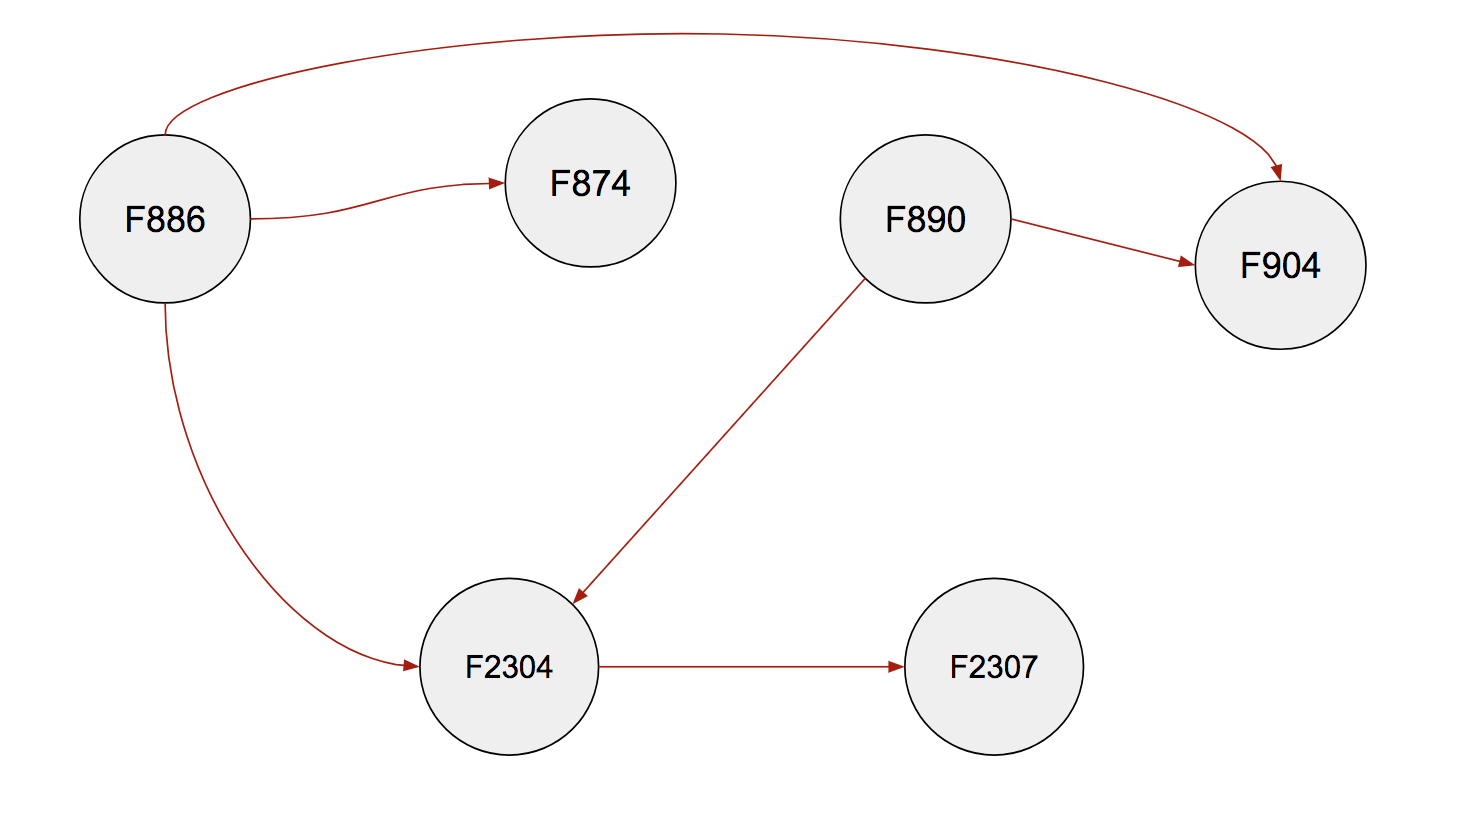
\includegraphics[width=15cm]{MasterThesis-master/f2f.png}\\
    \caption{Feasible paths between flight nodes}
    \label{fig:f2f}
\end{figure}

\begin{table}[h]
\renewcommand{\arraystretch}{1}
\caption{Feasible paths between flights and flights}
\label{Example Feasible paths f2f}
\begin{center}
\begin{tabular}{|c|c|c|c|c|c|c|}
\hline
\multicolumn{1}{|c|}{}
&\multicolumn{1}{|c|}{\(f886\)}
&\multicolumn{1}{c|}{\(f874\)}
&\multicolumn{1}{c|}{\(f890\)}
&\multicolumn{1}{c|}{\(f904\)}
&\multicolumn{1}{c|}{\(f2304\)}
&\multicolumn{1}{c|}{\(f2307\)}

\\  \hline
\(f886\) & 0 & 1 & 0 & 1 & 1 & 0
\\	\hline
\(f874\) & 0 & 0 & 0 & 0 & 0 & 0
\\	\hline
\(f890\) & 0 & 0 & 0 & 1 & 1 & 0
\\  \hline
\(f904\) & 0 & 0 & 0 & 0 & 0 & 0
\\  \hline
\(f2304\) & 0 & 0 & 0 & 0 & 0 & 1
\\  \hline
\(f2307\) & 0 & 0 & 0 & 0 & 0 & 0
\\  \hline
\end{tabular}
\end{center}
\end{table}

Secondly, we explore feasible path form aircraft to flights.
If aircraft \(a\) and flight \(f\) satisfy the following conditions, then there will be a feasible path from \(a\) to \(f\):
\begin{itemize}
    \item The current location of aircraft \(a\) is the same as flight \(f\) ’s departure airport;
    \item The departure time of flight\(f\) is later than the available time of aircraft \(a\);
    \item Aircraft \(a\) has required passenger seats of flight \(f\).
\end{itemize}
Using example data, the feasible paths from aircraft to flights can be represented by Fig\ref{fig:a2f}. And we also use a 0-1 table Table \ref{Example Feasible paths a2f} to record this relationship.

\begin{figure}[h]
    \centering
    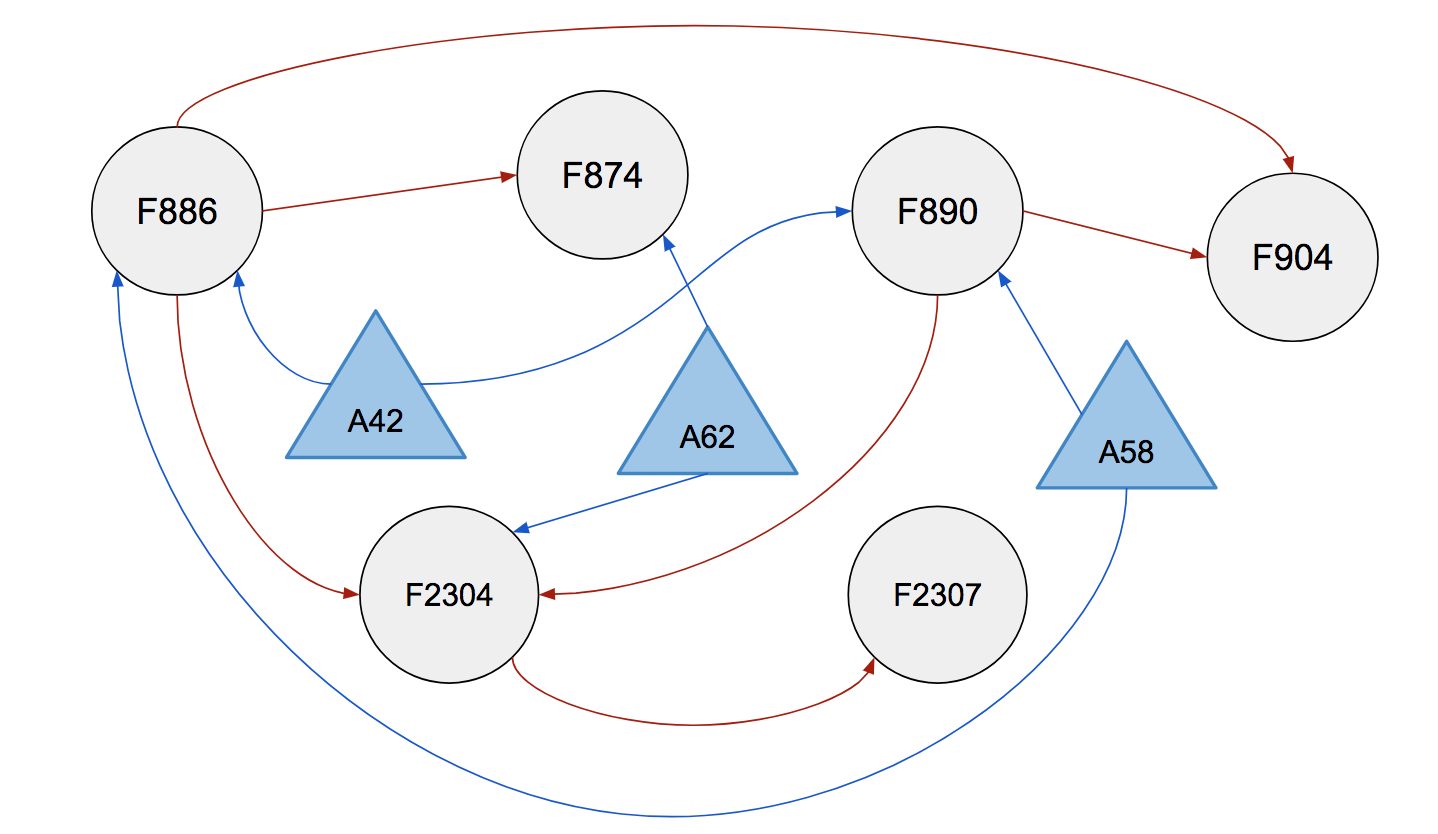
\includegraphics[width=15cm]{MasterThesis-master/a2f.png}\\
    \caption{Feasible path between aircraft nodes and flight nodes}
    \label{fig:a2f}
\end{figure}

\begin{table}[h]
\renewcommand{\arraystretch}{1}
\caption{Feasible path between aircraft nodes and flight nodes}
\label{Example Feasible paths a2f}
\begin{center}
\begin{tabular}{|c|c|c|c|c|c|c|}
\hline
\multicolumn{1}{|c|}{}
&\multicolumn{1}{|c|}{\(f886\)}
&\multicolumn{1}{c|}{\(f874\)}
&\multicolumn{1}{c|}{\(f890\)}
&\multicolumn{1}{c|}{\(f904\)}
&\multicolumn{1}{c|}{\(f2304\)}
&\multicolumn{1}{c|}{\(f2307\)}
\\  \hline
\(A42\) & 1 & 0 & 1 & 0 & 0 & 0
\\	\hline
\(A58\) & 1 & 0 & 1 & 0 & 0 & 0
\\	\hline
\(A62\) & 0 & 1 & 0 & 0 & 1 & 0
\\  \hline
\end{tabular}
\end{center}
\end{table}

\begin{figure}[h]
    \centering
    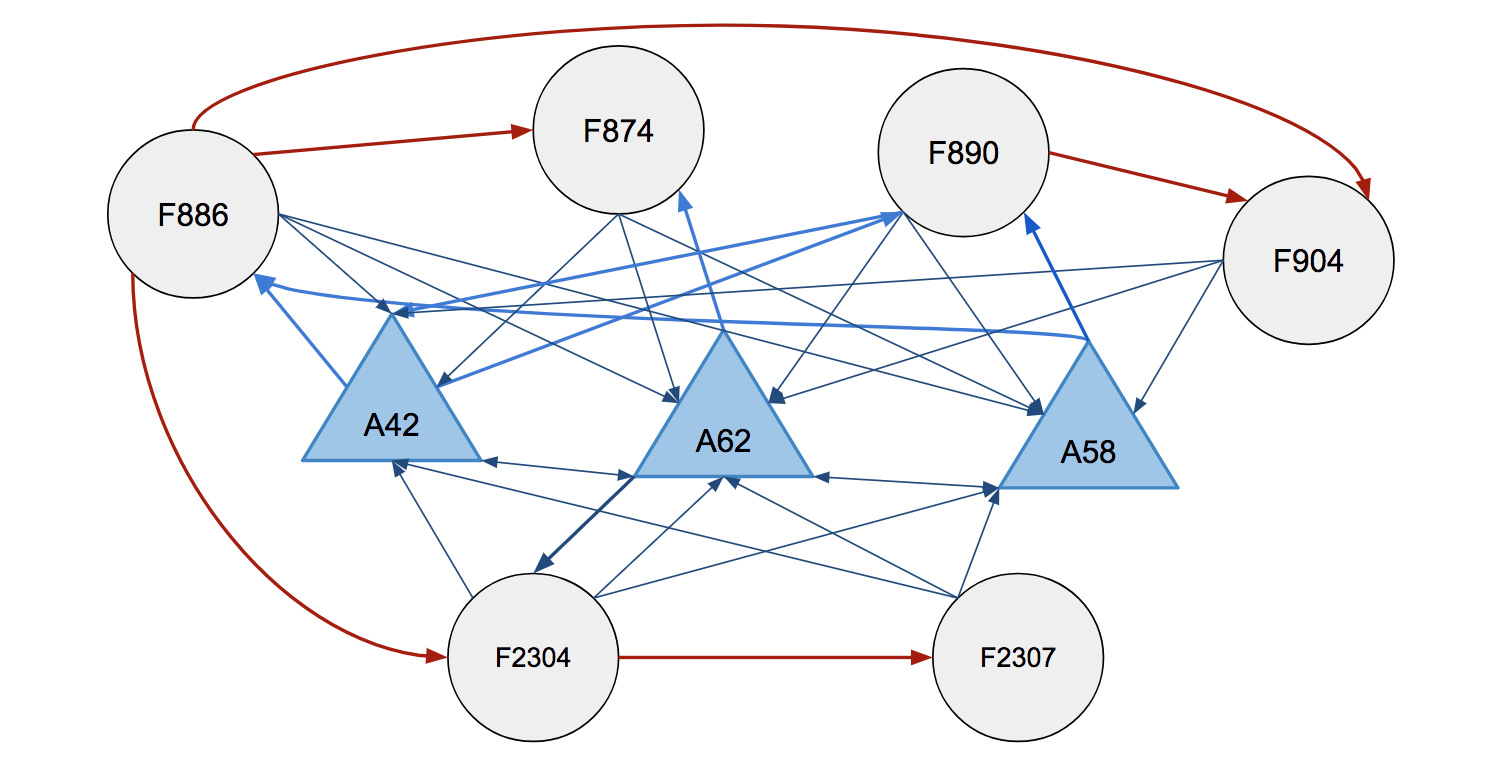
\includegraphics[width=15cm]{MasterThesis-master/completed web.png}\\
    \caption{All feasible paths}
    \label{fig:all feasible paths}
\end{figure}

And finally, in order to find one path that can go through all aircraft nodes, all the path should be linked together. So all the nodes(include aircraft and flights) has path to aircraft nodes in spite of their departure time or location. The Fig\ref{fig:all feasible paths} shows the completed web of all feasible paths based on original schedule. 
We use Table\ref{a2a & f2a} to represent the relationship between all nodes to aircraft nodes. And we merge Table\ref{fig:f2f},\ref{fig:a2f} and \ref{a2a & f2a}together to get Table\ref{all paths}.
This is the feasible paths between all nodes based on the original schedule. If there is any flight change happens, this table will be updated.

\begin{table}[h]
\renewcommand{\arraystretch}{1}
\caption{Feasible path to aircraft nodes}
\label{a2a & f2a}
\begin{center}
\begin{tabular}{|c|c|c|c|}
\hline
\multicolumn{1}{|c|}{}
&\multicolumn{1}{|c|}{\(A42\)}
&\multicolumn{1}{c|}{\(A58\)}
&\multicolumn{1}{c|}{\(A62\)}
\\  \hline
\(A42\) & 0 & 1 & 1
\\	\hline
\(A58\) & 1 & 0 & 1
\\	\hline
\(A62\) & 1 & 1 & 0 
\\  \hline
\(f886\) & 1 & 1 & 1
\\	\hline
\(f874\) & 1 & 1 & 1
\\	\hline
\(f890\) & 1 & 1 & 1
\\  \hline
\(f904\) & 1 & 1 & 1
\\  \hline
\(f2304\) & 1 & 1 & 1
\\  \hline
\(f2307\) & 1 & 1 & 1
\\  \hline
\end{tabular}
\end{center}
\end{table}

\begin{table}[h]
\renewcommand{\arraystretch}{1}
\caption{All feasible paths matrix}
\label{all paths}
\begin{center}
\begin{tabular}{|c|c|c|c|c|c|c|c|c|c|}
\hline
\multicolumn{1}{|c|}{}
&\multicolumn{1}{|c|}{\(A42\)}
&\multicolumn{1}{c|}{\(A58\)}
&\multicolumn{1}{c|}{\(A62\)}
&\multicolumn{1}{|c|}{\(f886\)}
&\multicolumn{1}{c|}{\(f874\)}
&\multicolumn{1}{c|}{\(f890\)}
&\multicolumn{1}{c|}{\(f904\)}
&\multicolumn{1}{c|}{\(f2304\)}
&\multicolumn{1}{c|}{\(f2307\)}
\\  \hline
\(A42\) & 0 & 1 & 1 & 1 & 0 & 1 & 0 & 0 & 0
\\	\hline
\(A58\) & 1 & 0 & 1 & 1 & 0 & 1 & 0 & 0 & 0
\\	\hline
\(A62\) & 1 & 1 & 0 & 0 & 1 & 0 & 0 & 1 & 0
\\  \hline
\(f886\) & 1 & 1 & 1 & 0 & 1 & 0 & 1 & 1 & 0
\\	\hline
\(f874\) & 1 & 1 & 1 & 0 & 0 & 0 & 0 & 0 & 0
\\	\hline
\(f890\) & 1 & 1 & 1 & 0 & 0 & 0 & 1 & 1 & 0
\\  \hline
\(f904\) & 1 & 1 & 1 & 0 & 0 & 0 & 0 & 0 & 0
\\  \hline
\(f2304\) & 1 & 1 & 1 & 0 & 0 & 0 & 0 & 0 & 1
\\  \hline
\(f2307\) & 1 & 1 & 1 & 0 & 0 & 0 & 0 & 0 & 0
\\  \hline
\end{tabular}
\end{center}
\end{table}

Now we insert some disruption.
Suppose that \(f886\) is delayed for a long time, so the path between \(f886\) and \(f874\) is not feasible. The feasible paths changes shows in Fig\ref{fig:disruption}. 
And we also update Table\ref{all paths} to Table\ref{table:updated paths}. 
\begin{figure}[h]
    \centering
    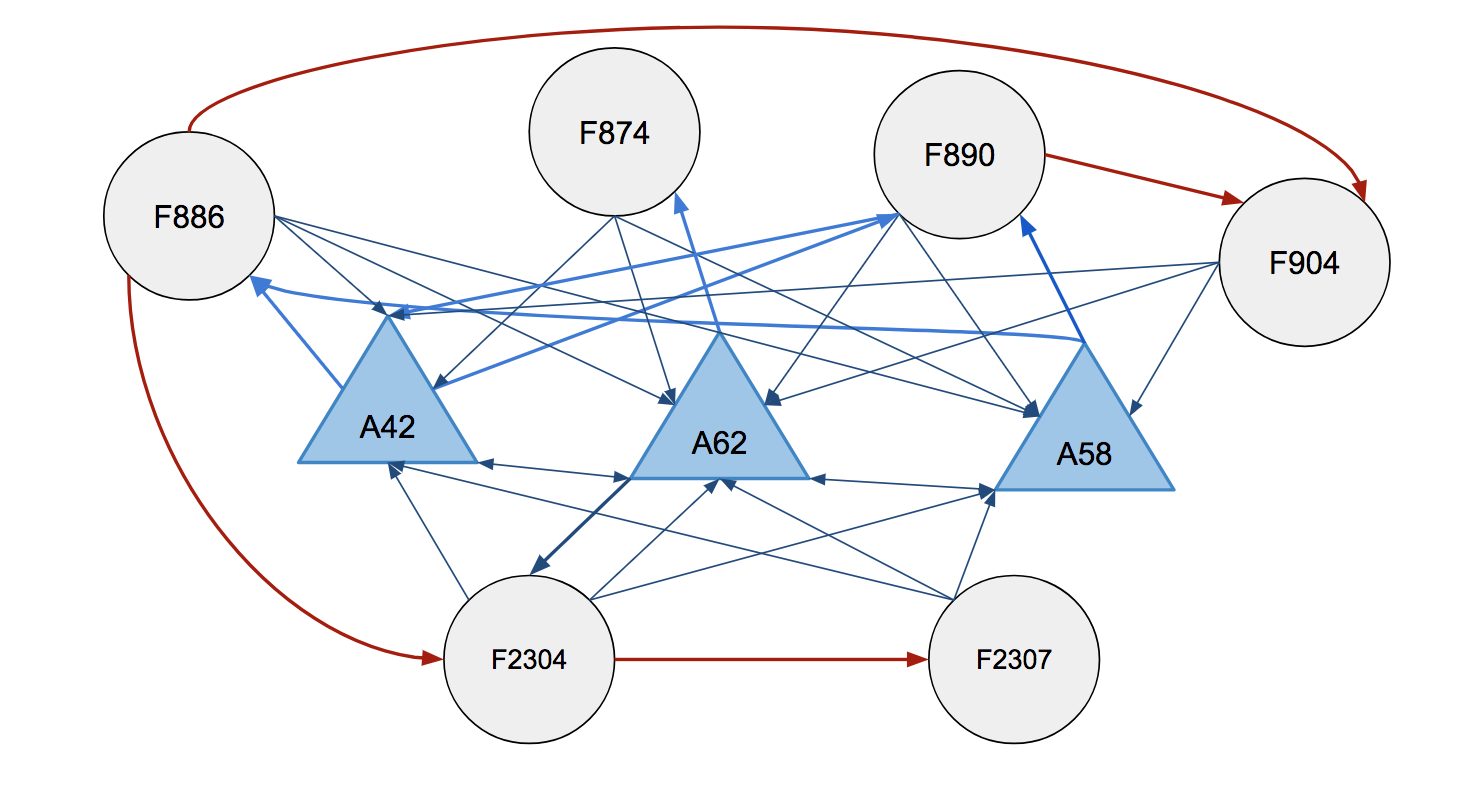
\includegraphics[width=15]{MasterThesis-master/updated paths.png}
    \caption{Update feasible path after disruption}
    \label{fig:disruption}
\end{figure}

\begin{table}[h]
\renewcommand{\arraystretch}{1}
\caption{Updated paths matrix}
\label{table:updated paths}
\begin{center}
\begin{tabular}{|c|c|c|c|c|c|c|c|c|c|}
\hline
\multicolumn{1}{|c|}{}
&\multicolumn{1}{|c|}{\(A42\)}
&\multicolumn{1}{c|}{\(A58\)}
&\multicolumn{1}{c|}{\(A62\)}
&\multicolumn{1}{|c|}{\(f886\)}
&\multicolumn{1}{c|}{\(f874\)}
&\multicolumn{1}{c|}{\(f890\)}
&\multicolumn{1}{c|}{\(f904\)}
&\multicolumn{1}{c|}{\(f2304\)}
&\multicolumn{1}{c|}{\(f2307\)}
\\  \hline
\(A42\) & 0 & 1 & 1 & 1 & 0 & 1 & 0 & 0 & 0
\\	\hline
\(A58\) & 1 & 0 & 1 & 1 & 0 & 1 & 0 & 0 & 0
\\	\hline
\(A62\) & 1 & 1 & 0 & 0 & 1 & 0 & 0 & 1 & 0
\\  \hline
\(f886\) & 1 & 1 & 1 & 0 & \textcolor{red}{0} & 0 & 1 & 1 & 0
\\	\hline
\(f874\) & 1 & 1 & 1 & 0 & 0 & 0 & 0 & 0 & 0
\\	\hline
\(f890\) & 1 & 1 & 1 & 0 & 0 & 0 & 1 & 1 & 0
\\  \hline
\(f904\) & 1 & 1 & 1 & 0 & 0 & 0 & 0 & 0 & 0
\\  \hline
\(f2304\) & 1 & 1 & 1 & 0 & 0 & 0 & 0 & 0 & 1
\\  \hline
\(f2307\) & 1 & 1 & 1 & 0 & 0 & 0 & 0 & 0 & 0
\\  \hline
\end{tabular}
\end{center}
\end{table}


\section{Ant Colony optimization implement}
When disruption break the original schedule, we intercept the flights suffered with break and aircraft still available then generate flight information dataset and aircraft status dataset. Using approach mentioned in last section, get feasible path matrix which involves value 0-1. 
Before start ant colony iteration, we need to generate a 
pheromone matrix which is an identity matrix.
At beginning, the first node that ant chooses must be the aircraft node. That means each route starts at an aircraft.

Ants choose the next node by the probability calculated by Func.\ref{probability}. In this part, we will use both pheromone matrix and feasible path matrix.
The role of feasible path matrix is used as a heuristic factor. This matrix let probability of unfeasible path be 0 so that ants won't choose those path. And use feasible path matrix and pheromone matrix separately make it more easier to add modification on pheromone matrix. Changing pheromone globally will not influence the feasibility of paths.

After a group of ants all finish one iteration and create a completed route. We calculate the fitness which is the total cost in this model, and record the least one as well as the path of the least one. Then using reciprocal of this least fitness as change quantity:
\begin{equation}\label{func:delta pheromone}
    \Delta\rho = C * \left( \frac{1}{Total\_cost} \right)
\end{equation}
\(C\) is a constant to rationalize reciprocal of total cost because if $\frac{1}{Total\_cost}$ is too small, the pheromone matrix will be nearly no changed. Then we update pheromone matrix globally. 
\begin{equation}
    new\ \rho_k = max(1, \rho_k * (1-\mu) + \Delta\rho)
\end{equation}
Pheromone concentration should no less than original concentration 1. Because at a couple of iteration at beginning, the path is chosen randomly. So if some path is not be selected at first, their pheromone concentration still evaporate during iteration, then they will have less and less chance to be selected. So let the minimum value of pheromone concentration on each path can avoid this kind of problem.

\section{Fitness calculation}\label{Fitness calculation}

 In this model, we use total cost as fitness, just same as the total distance in traveling salesman problem. But when we get a completed path, a sequence list of aircraft and flights, how to transfer it into cost? We also use the example of Section\ref{Section4.2} to explain.

Suppose that Fig is one feasible solution. From this we can get a sequence list.

\begin{figure}[h]
    \centering
    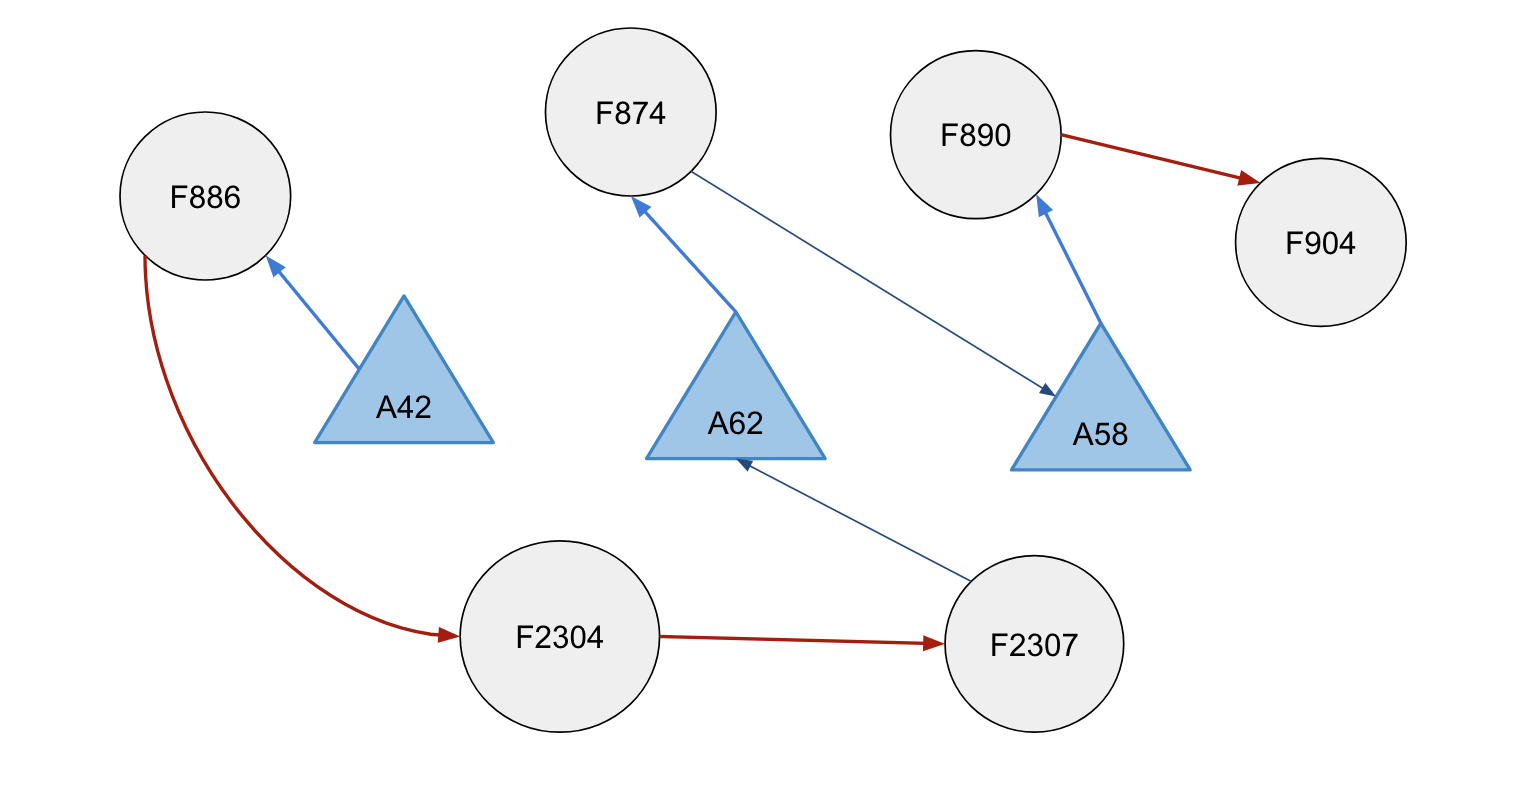
\includegraphics[width=10]{MasterThesis-master/feasible solution1.png}
    \caption{One feasible solution}
    \label{fig:one feasible solution}
\end{figure}

\begin{table}[h]
\renewcommand{\arraystretch}{1.2}
\caption{Feasible Solution}
\label{outcome}
\begin{center}
\begin{tabular}{|c|c|c|c|c|c|c|c|c|}
\hline 
\multicolumn{1}{c|}{\(A42\)}
&\multicolumn{1}{c|}{\(f886\)}
&\multicolumn{1}{c|}{\(f2304\)}
&\multicolumn{1}{c|}{\(f2307\)}
&\multicolumn{1}{c|}{\(A62\)}
&\multicolumn{1}{c|}{\(f874\)}
&\multicolumn{1}{c|}{\(A58\)}
&\multicolumn{1}{c|}{\(f890\)}
&\multicolumn{1}{c|}{\(f904\)}\\
\hline
\end{tabular}
\end{center}
\label{piriform fscore}
\end{table}

\begin{table}[h]
\renewcommand{\arraystretch}{1.2}
\caption{Original Schedule}
\label{outcome}
\begin{center}
\begin{tabular}{|c|c|c|c|c|c|c|c|c|}
\hline 
\multicolumn{1}{c|}{\(A42\)}
&\multicolumn{1}{c|}{\(f886\)}
&\multicolumn{1}{c|}{\(f874\)}
&\multicolumn{1}{c|}{\(A62\)}
&\multicolumn{1}{c|}{\(f2304\)}
&\multicolumn{1}{c|}{\(f2307\)}
&\multicolumn{1}{c|}{\(A58\)}
&\multicolumn{1}{c|}{\(f890\)}
&\multicolumn{1}{c|}{\(f904\)}\\
\hline
\end{tabular}
\end{center}
\label{piriform fscore}
\end{table}

We can 

\subsection{ISBI 2012 EM Segmentation Dataset}
The other dataset for neuronal boundary detection in EM images is the ISBI 2012 EM Segmentation Dataset. As the dataset for the popular ISBI 2012 EM Segmentation Challenge, ISBI 2012 EM Segmentation Dataset does not offer the ground-truth segmentation for the testing stack, which is reasonable but increases the difficulty of results analyzing and discussion. Besides, the raw training data with annotations are relatively insufficient, where there is only one stack for training with the dimension of 30 \(\times\) 512 \(\times\) 512. To train a very deep network using such a few images is theoretically difficult, even though we use the standard data augmentation to enrich the training materials. 

Network settings are the same as ones we used in the experiment for Mouse Piriform Cortex Dataset\cite{Lee2015}. Standard data augmentation (Section \ref{experiment of piriform}) is considered here, too.

The Rand F-score data from the leaderboard of ISBI 2012 EM Segmentation Challenge are shown in Table \ref{isbi12 fscore} . Not all the scores are presented since there are many entries in the leaderboard which have not been reported in literature. It worths noting that most of the leading methods apply post-processing algorithms or assemble several models to improve the ranking. However, the proposed cascaded networks without any post-processing procedures can achieve competitive result to those with post-processing. 
The post-processing used in each approach is also presented in Table \ref{isbi12 fscore}, where \cite{Beier2016} is a post-processing algorithm itself and can be adopted to ours. With a proper post-processing, our network can win the state-of-the-art with more powerful ResNet\cite{He2016} as its base network. In the future, we will embed the ResNet\cite{He2016} in our cascaded framework to further improve the performance.


\begin{table}[t]
\renewcommand{\arraystretch}{0.8}
\caption{The Rand F-scores part from the leaderboard of ISBI 2012 EM Segmentation Challenge\cite{Ronneberger2015}.}
\label{outcome}
\begin{center}
\begin{tabular}{|c|c|}
\hline
&\multicolumn{1}{c|}{Rand F-score}\\
\hline
U-net\cite{Ronneberger2015} 			& 0.9727	\\	\hline
CUMedVision\cite{Chen2016} 			& 0.9768 	\\	\hline
IAL IC\cite{Beier2016}			& 0.9773	 \\	\hline
FusionNet\cite{Quan2016} 			& 0.9780	\\	\hline
Ours(3-stage) 			& 0.9780	\\	\hline
PolyMtl\cite{Drozdzal2017} 			& 0.9806	\\	\hline
Ours(3-stage) + IAL IC			& 0.9836	\\	\hline
\end{tabular}
\end{center}
\label{isbi12 fscore}
\end{table}



\section{Object Boundary Detection in Natural Images}

\begin{figure}[t]
  \centering
  % Requires \usepackage{graphicx}
  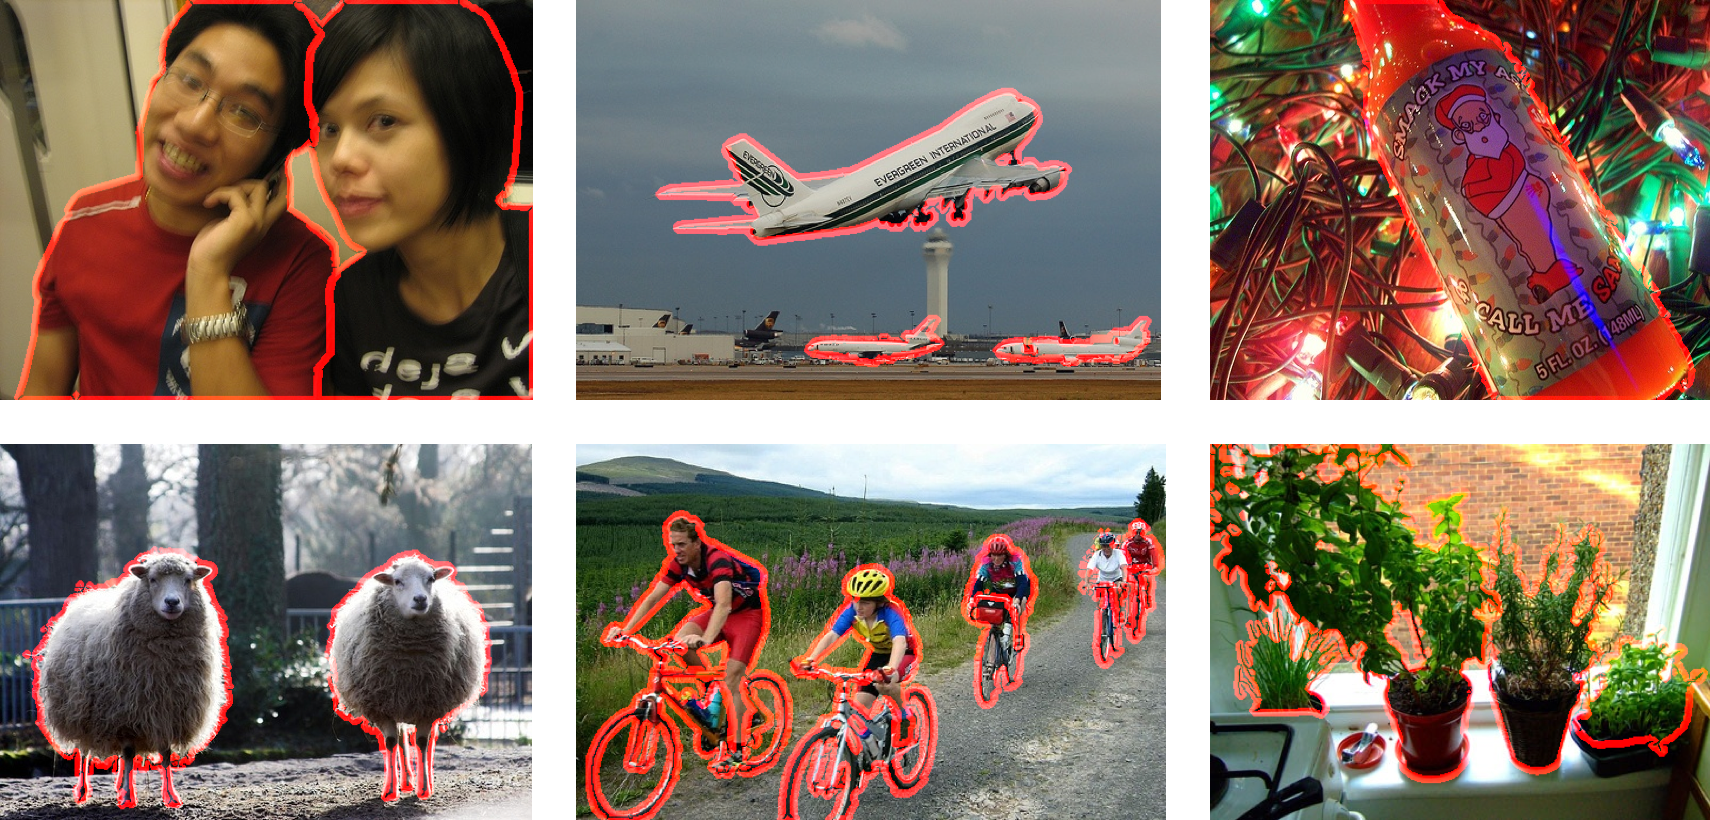
\includegraphics[width=15cm]{voc_contour.png}\\
  \caption{Examples selected from PASCAL VOC Contour Dataset\cite{Yang2016}, where ground-truth contours are labeled as red. There are various objects (human, artificialities, animals, plants, etc.) appearing in complex scenes (indoor and outdoor environments, colorful backgrounds, blurs, textural confusions, etc), which significantly increases the difficulty of detecting the object-level boundary.}\label{voc contour}
\end{figure}

Our work begins at Neuronal Boundary Detection of EM images but dose not end in it. By applying the proposed multi-stage network to common object boundary detection in natural images, we evaluate the generalization capacity of our network.

\subsection{Metrics}
Precision and Recall are the well-accepted metrics for two-class annotation tasks\cite{Shen2016CVPR, Shen2017TIP, Yang2016}. Given the notations as follows: 
(1) True Positive \emph{(TP)}: the times of annotating a positive pixel as positive;
(2) False Positive \emph{(FP)}: the times of annotating a negative pixel as positive;
(3) True negative \emph{(TN)}: the times of annotating a negative pixel as negative;
(4) False positive \emph{(FN)}: the times of annotating a positive pixel as negative;
we have Precision \emph{(P)}, Recall \emph{(R)} and their harmonic average F-measure

\begin{eqnarray}
P &=& \frac{TP}{TP+FP} \\
R &=& \frac{TP}{TP+FN} \\
F-measure &=& \frac{2PR}{P+R} \\
\end{eqnarray}

The Precision-Recall Curve \emph(PR-curves) can be also generated by varying the threshold for boundary binarization\cite{Shen2016CVPR}.

\subsection{PASCAL VOC Contour Dataset}
PASCAL VOC Segmentation Datasets are a series of well-accepted object segmentation datasets,  including the well-annotated natural photos released from 2007 to 2012. \cite{Yang2016} apply DenseCRF\cite{Krahenbuhl2011} to further refine the boundary annotation from the segmentation ground-truth and release a large instance-level object boundary detection dataset, PASCAL VOC Contour Dataset, with 10582 training images, 1449 testing images and their corresponding boundary annotations. Different from EM images, these natural photos are taken from various scenes and contain kinds of objects (Fig. \ref{voc contour}). For example, in each photo, the image scale, the number and category of the object are different. There are also many samples with blurred object boundary and confused background on the dataset. All these significantly increase the difficulty of boundary detection on the PASCAL VOC Contour Dataset, while call out a deep network with sufficient capacity to extract the highly abstract object-level features from the data.

With such a large dataset, the standard data augmentation with a ratio of 36 is not necessary nor efficient. We follow the light-weight data augmentation mentioned in \cite{Yang2016}, by randomly cropping four 224 \(\times\) 224 patches from the raw image and flipping them once, resulting in 8\(\times\) training samples. Here, the cropping is mainly for memory efficiency\cite{Yang2016} and the mini-batch based training. Original FCNs\cite{Long2015} is not available for the training with multiple training samples in one mini-batch, because these samples may have different scales and can result in error. By fixing the cropped patches into one-size, we are able to enlarge the batch-size, 8 in practice, for a more effective and faster training.

We fine-tune the proposed network on PASCAL VOC Contour Dataset using the same strategy in Section \ref{experiment of piriform}. Firstly, we train a single-stage network with the same structure as HED\cite{Xie2015}. Then we use the fine-tuned HED network to initialize the training for our 2-stage and 3-stage cascaded fully convolutional networks. F-measure comparisons are shown in \ref{voc fscore}. 

For optimization, we use the standard Stochastic Gradient Descent \emph{(SGD)}. Other hyper parameters such as the level of convolution in each subnet, learning rate, momentum and weight decay are same as what we used in the experiments of neuronal boundary detection. As demonstrated in \cite{Yang2016}, to process all the training samples, named one epoch, takes around 10000 iterations. We train the single-stage, 2-stage and 3-stage networks for 2 epochs, 4 epochs, and 5 epochs respectively. Compared with the CEDN proposed in \cite{Yang2016}, the training for our cascaded networks costs only half of the time for training CEDN, which proves the effectiveness of the proposed recursively end-to-end training.

As we expected, traditional methods for local edge detection such as SCG, its multi-scale version MCG\cite{Arbelaez2014}, and Structured Random Forest for Edge Detection \emph{(SE)}\cite{Dollar2013} present poor results on this benchmark. These methods use hand-crafted features which often combine multiple cues like color, brightness, spectrum, to handle different cases. HED\cite{Xie2015} has the ability to naturally obtain the hierarchical features due to the adoption of the holistically-nested network, which is also used in our sub-networks. We fine-tune it on PASCAL VOC Contour Dataset and receive a F-measure of 0.52, much better than the traditional methods but lower than our 2-stage network. What's more, our 3-stage network outperforms CEDN\cite{Yang2016} by 2\% and achieves the state-of-the-art score on this benchmark. PR-curves in Fig. \ref{voc prcurve} illustrate the refinement benefits from the cascaded network structure.

\begin{table}[t]
\renewcommand{\arraystretch}{0.8}
\caption{Object boundary detection evaluation comparison on PASCAL VOC Contour Dataset\cite{Yang2016}. Our proposed 3-stage cascaded fully convolutional network achieves the new state-of-the-art on this benchmark, with a significant improvement (around 2\% over the second)).}
\label{outcome}
\begin{center}
\begin{tabular}{|c|c|}
\hline
&\multicolumn{1}{c|}{F-measure}\\
\hline
SCG\cite{Arbelaez2014} 			& 0.36	\\	\hline
MCG\cite{Arbelaez2014} 			& 0.37 	\\	\hline
SE\cite{Dollar2013}			& 0.37	 \\	\hline
HED\cite{Xie2015} 			& 0.52	\\	\hline
Ours(2-stage) 			& 0.53	\\	\hline
CEDN\cite{Yang2016}		& 0.57	\\	\hline
\textbf{Ours(3-stage)} 	& \textbf{0.59}	\\	\hline
\end{tabular}
\end{center}
\label{voc fscore}
\end{table}

\begin{figure}[t]
  \centering
  % Requires \usepackage{graphicx}
  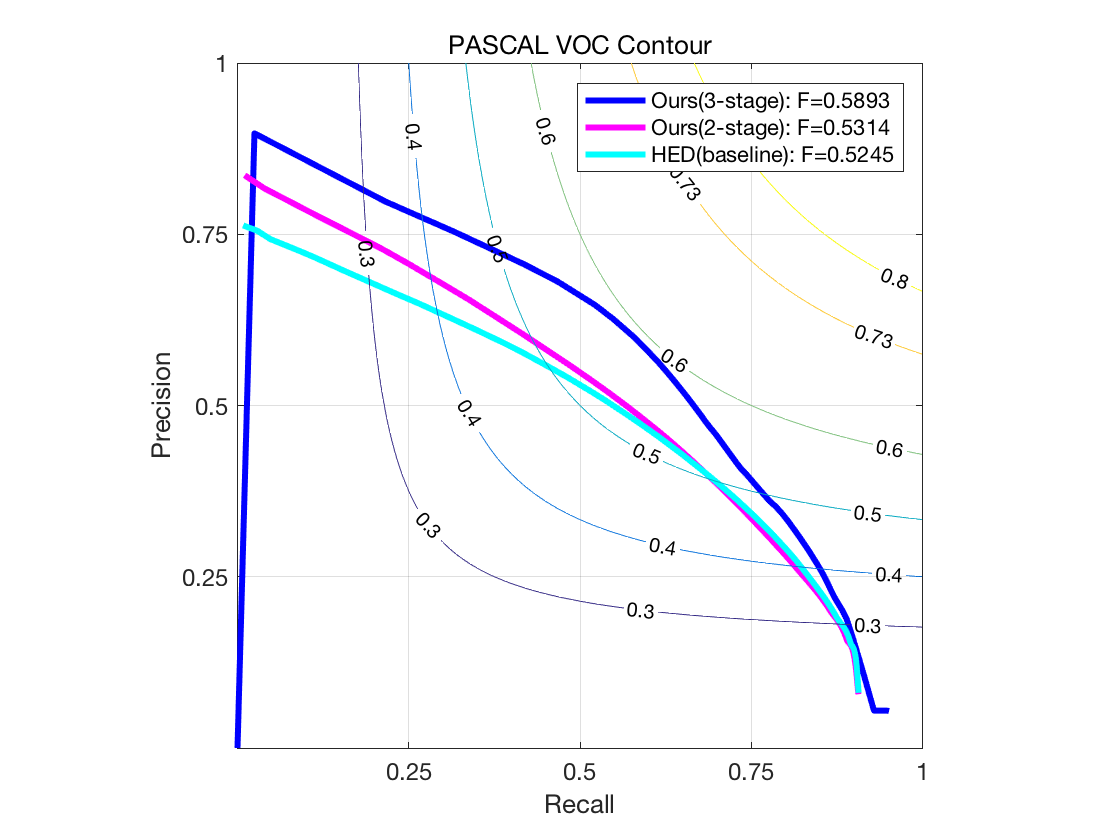
\includegraphics[width=15cm]{voc_prcurve.png}\\
  \caption{Precision-recall curves on PASCAL VOC Contour Dataset\cite{Yang2016}.}\label{voc prcurve}
\end{figure}

\section{Control Experiments for Model Interpretation}3

To verify the explaination and interpretation in Section \ref{interpretation}, we design a series of control experiments and give the neuronal boundary detection evaluation on Mouse Piriform Cortex Dataset\cite{Lee2015}. We do not test on the ISBI 2012 Segmentation Dataset\cite{Ronneberger2015} since there is no provided annotation for testing images on it. 

There are three control experiments, for which we design eight kind of networks with different network structures:

$\bullet$ \textbf{Baseline} HED\cite{Xie2015} pre-trained on BSDS 500 Dataset\cite{Arbelaez2011}

$\bullet$ \textbf{Nerwork A} 1-stage (HED\cite{Xie2015}) network with 5 levels in one stage, end-to-end training and no recursive input;

$\bullet$ \textbf{Network B} 2-stage cascaded network with 4 levels in each stage, end-to-end training and multi-recursive-input;

$\bullet$ \textbf{Network C} 2-stage cascaded network with 5 levels in each stage, end-to-end training and multi-recursive-input;

$\bullet$ \textbf{Network D} 3-stage cascaded network with 5 levels in each stage, end-to-end training and multi-recursive-input;

$\bullet$ \textbf{Network E} 2-stage cascaded network with 5 levels in each stage, end-to-end training and single-recursive-input (only the level 4);

$\bullet$ \textbf{Network F} 2-stage cascaded network with 5 levels in each stage, end-to-end training and single-recursive-input (only the level 5);

$\bullet$ \textbf{Network G} 2-stage cascaded network with 5 levels in each stage, stepwise training and multi-recursive-input;


\subsection{Evaluations on Cascaded Architecture \emph{vs.} Single-stage Architecture}

\begin{table}[t]
\renewcommand{\arraystretch}{0.6}
\caption{Control Experiment 1: Cascaded Architecture \emph{vs.} Single-stage Architecture}
\label{outcome}
\begin{center}
\begin{tabular}{|c|c|}
\hline
&\multicolumn{1}{c|}{Rand F-score}\\
\hline
Baseline 			& 0.9680	\\	\hline
Network A 		& 0.9688 	\\	\hline
Network B			& 0.9739	 \\	\hline
Network C 		& 0.9819	\\	\hline
Network D 		& 0.9866	\\	\hline
\end{tabular}
\end{center}
\label{control experiment 1}
\end{table}

To prove the proposed cascaded architecture effective in boundary detection, we compare our 2-stage (Network C) and 3-stage (Network E) cascaded networks with a 1-stage fine-tuned HED\cite{Xie2015} network (Network A) and the baseline HED\cite{Xie2015} pre-trained on a local edge boundary detection dataset, BSDS 500\cite{Arbelaez2011}. Results show that even a 2-stage cascaded network with only 4 convolution levels outperforms the baseline and the single-stage fine-tuned network with 5 convolution levels. If we stack more sub-networks while controlling the rest hyper-parameters, we can find the performance boosting from 0.9688 (Network A), to 0.9819 (Network C) and 0.9866 (Network D) step by step (Table \ref{control experiment 1}), which indicates that the proposed cascaded structures effective in high-level object boundary detection. The improvement achieved by stepwise removing the confounding local edges inside the objects (circuits), and refining the boundary with low contrast to the non-boundary area, illustrated by Fig. \ref{control 1}.

\begin{figure}[t]
  \centering
  % Requires \usepackage{graphicx}
  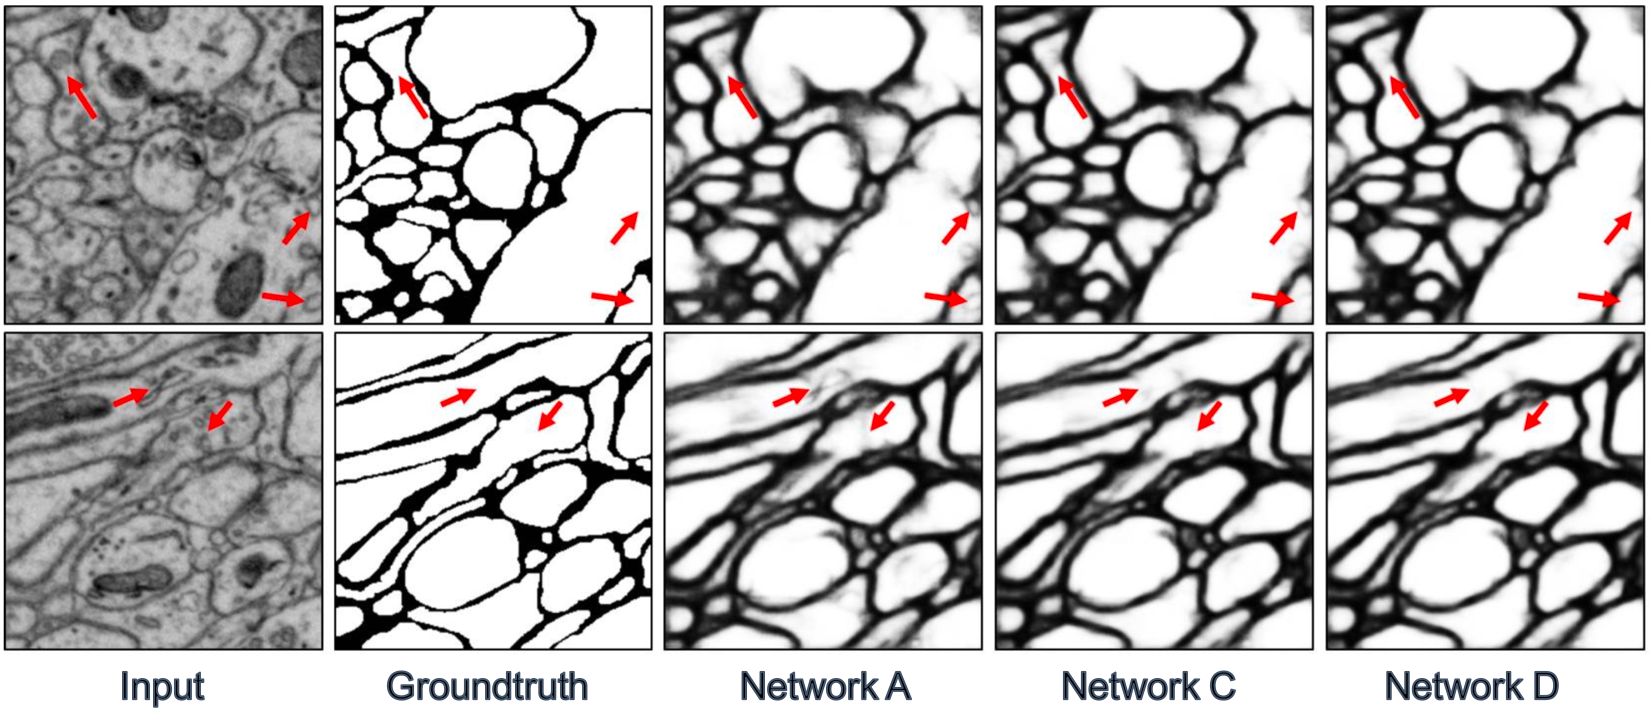
\includegraphics[width=15cm]{control_1.png}\\
  \caption{Qualitative examples to reveal how cascaded networks improve the high-level boundary detection result. For example, the arrows mean the false positive detections are removed step by step.}\label{control 1}
\end{figure}

\subsection{Evaluations on Multi-recursive-input vs. Single-recursive-input}

\begin{table}[t]
\renewcommand{\arraystretch}{0.6}
\caption{Control Experiment 2: Multi-recursive-input vs. Single-recursive-input}
\label{outcome}
\begin{center}
\begin{tabular}{|c|c|}
\hline
&\multicolumn{1}{c|}{Rand F-score}\\
\hline
Network F 		& 0.9410 	\\	\hline
Network E			& 0.9656	 \\	\hline
Baseline	 		& 0.9680	\\	\hline
Network C 		& 0.9819	\\	\hline
\end{tabular}
\end{center}
\label{control_experiment_2}
\end{table}

As we mentioned in Section {interpretation}, Multi-recursive-input plays a important role in the high-level object boundary detection, by providing the multi-scale features in a natural way. In order to evaluate it, we design several 2-stage single-recursive-input networks (Network E, F) and compare them with our 2-stage multi-recursive-input network (Network C). Cause we do not know which level is the best for inputing to the next stage, we input the level 4 (in Network E) and level 5 (in Network F) to the next sub-network respectively. According to Table \ref{control_experiment_2}, we surprisingly find the cascaded networks with single-recursive-input perform bad even when comparing with the pre-trained 1-stage network (Baseline). The single-recursive-input from the previous stage has only the features in one scale, either large or small. If we only feed the large-scale features with low-resolution into the next stage, there will be the a huge loss in image details. If we only feed the small-scale features into the next stage, the cascaded structure will be deprecated. It is always a hard problem for people to choose a best level as the recursive input, so we highlight the multi-recursive-input again in the cascaded structures.

\subsection{Evaluations on End-to-end Training vs. Stepwise Self-tuning}

\begin{table}[t]
\renewcommand{\arraystretch}{0.6}
\caption{Control Experiment 3: End-to-end Training vs. Stepwise Self-tuning}
\label{outcome}
\begin{center}
\begin{tabular}{|c|c|}
\hline
&\multicolumn{1}{c|}{Rand F-score}\\
\hline
Baseline	 		& 0.9680	\\	\hline
Network G 		& 0.9762	\\	\hline
Network C 		& 0.9819	\\	\hline
\end{tabular}
\end{center}
\label{control_experiment_3}
\end{table}

In the end, we design a control experiment with only the training strategy varied to see whether our cascaded networks benefit from the end-to-end training or not. As shown in Table \ref{control_experiment_3}, the cascaded network trained end-to-end (Network C) outperforms the same network but trained stepwise (Network G). The end-to-end training was hardly used to learn such a deep network, due to the consideration of gradient vanishing. However, the holistically-nested sub-networks and multi-recursive-input release the limitation, which enables the end-to-end training in our deep cascaded networks. 

\chapter{Conclusions} \label{conclusions}

Object-level boundary is a useful but unexplored topic in computer vision. With a well-detected object boundary, the segment of the object will be easily extracted, which can be applied for object proposal, shape based object recognition and  kinds of object detection problems. Based on the previous works in neuronal boundary detection, we develop a series of cascaded fully convolutional networks to detection high-level boundary in EM images. Not end up with the improvement achieved in EM images, we further extend the cascaded architecture to the object boundary detection in natural images, and design several control experiments to interpret how it works. Our model is proved to be both effective and interpretable in various boundary detection scenes, thus easy to be aggregated with other frameworks.

In the future, we will try some other structures for the alternative sub-networks, such as the recent published Richer Convolutional Features for Edge Detection\cite{Liu2017}, which is now the state-of-the-art on many edge detection benchmarks. Applications of our object-level boundary detection can be also considered, such as the boundary-based object proposal\cite{Yang2016}. 







\bibliographystyle{IEEEtran}
\bibliography{LUOreference}


\end{document}
